\documentclass[a4paper, twoside]{report}

\usepackage[british]{babel}
\usepackage[T1]{fontenc}
\usepackage{listings}
\usepackage{hyperref}
\usepackage{multirow}
\usepackage{enumitem}
\usepackage[backend=biber,style=numeric-comp,sorting=none,maxcitenames=2]{biblatex}
\usepackage{url}
\addbibresource{Project.bib}
\usepackage{csquotes}
\usepackage{bookmark}
\DefineBibliographyExtras{british}{\def\finalandcomma{\addcomma}}
\renewbibmacro*{doi+eprint+url}{%
    \printfield{doi}%
    \newunit\newblock%
    \iftoggle{bbx:eprint}{%
        \usebibmacro{eprint}%
    }{}%
    \newunit\newblock%
    \iffieldundef{doi}{%
        \usebibmacro{url+urldate}}%
        {}%
    }

\usepackage[justification=centering]{caption}
%paragraph indentation
\setlength{\parindent}{4em} 
%paragraph spacing
\setlength{\parskip}{0.15em}
%Line spacing
\renewcommand{\baselinestretch}{1.5}
\usepackage{lscape}
\usepackage{color}
\usepackage{float}
\usepackage{adjustbox}
\hypersetup{colorlinks=false}
\usepackage{subfigure}
\usepackage{amsmath}
\newcommand{\R}{\mathbb{R}}
\newcommand{\Z}{\mathbb{Z}}
\newcommand{\Q}{\mathbb{Q}}
\newcommand{\N}{\mathbb{N}}
\newcommand{\s}{\sum_{n=1}^{\infty}}
\newcommand{\p}{\ensuremath{^{+}}}
\newcommand{\ps}{\ensuremath{^{+\gls*{sl}}}}
\newcommand{\ssl}{\ensuremath{_{\gls*{sl}}}}
\newcommand{\pw}{\ensuremath{^{+\gls*{wv}}}}
\newcommand{\ww}{\ensuremath{_{\gls*{wv}}}}
\newcommand{\pz}{\ensuremath{^{+\gls*{zer}}}}
\newcommand{\zz}{\ensuremath{_{\gls*{zer}}}}
\newcommand{\Ai}{\operatorname{Ai}}
\newcommand{\sct}{\textcite{chernyshenko2013}}
\newcommand{\scc}{\cite{chernyshenko2013}}
\newcommand{\vqt}{\textcite{viotti2009}}
\newcommand{\vqc}{\cite{viotti2009}}
\newcommand{\sgt}{\textcite{ghebali2017}}
\newcommand{\sgc}{\cite{ghebali2017}}
\newcommand{\lut}{\textcite{luchini1996}}
\newcommand{\luc}{\cite{luchini1996}}
\newcommand\Rey{\mbox{\textit{Re}}}  % Reynolds number
\newcommand\Pran{\mbox{\textit{Pr}}} % Prandtl number, cf TeX's \Pr product
\newcommand\Pen{\mbox{\textit{Pe}}}  % Peclet number
\usepackage{import}
\usepackage{cancel}
\usepackage{graphicx}
\usepackage{textcomp}
\usepackage[colorinlistoftodos]{todonotes}
\usepackage{siunitx}
\usepackage{physics}
\usepackage{pdfpages}
\usepackage{listings}
\usepackage{color} %red, green, blue, yellow, cyan, magenta, black, white
\definecolor{mygreen}{RGB}{28,172,0} % color values Red, Green, Blue
\definecolor{mylilas}{RGB}{170,55,241}
\usepackage[toc,acronyms,nomain,nonumberlist]{glossaries}
\newglossary[nlg]{notation}{not}{ntn}{Notation}
\usepackage{etoolbox}
\patchcmd{\abstract}{\titlepage}{}{}{}
\patchcmd{\endabstract}{\endtitlepage}{}{}

%% Sets page size and margins
\usepackage[a4paper,top=3cm,bottom=2cm,left=3cm,right=3cm,marginparwidth=2cm]{geometry}

\title{Semi-Empirical Optimisation of the Shape of a Surface Reducing Turbulent Skin Friction}
\author{Herman (Hon Man) Mak}
% Update supervisor and other title stuff in title/title.tex

%Glossary

\makenoidxglossaries
\newglossaryentry{re}
{
	type=notation,
	name={\ensuremath{\mbox{\textit{Re}}}},
	description={Reynolds number, and is equal to $\frac{U L}{\nu}$, a characteristic velocity $U$ multiplied by a characteristic length $L$ divided by kinematic viscosity $\nu$},
	sort={Re}
}
\newglossaryentry{ret}
{
	type=notation,
	name={\ensuremath{\mbox{\textit{Re}}_{\tau}}},
	description={friction Reynolds number, defined using friction velocity $u_\tau$ and channel half height $h$ as the characteristic velocity and length respectively},
	sort={Retau}
}
\newglossaryentry{hgt}
{
	type=notation,
	name={\ensuremath{h}},
	description={channel half height},
	sort={h}
}
\newglossaryentry{nu}
{
	type=notation,
	name={\ensuremath{\nu}},
	description={kinematic viscosity, defined as the ratio between dynamic viscosity and density $\frac{\mu}{\rho}$},
	sort={zznu}
}
\newglossaryentry{mu}
{
	type=notation,
	name={\ensuremath{\mu}},
	description={dynamic viscosity},
	sort={zzmu}
}
\newglossaryentry{ro}
{
	type=notation,
	name={\ensuremath{\rho}},
	description={fluid density},
	sort={zzrho}
}
\newglossaryentry{garea}
{
	type=notation,
	name={\ensuremath{A_g^{+}}},
	description={riblet groove area in wall units},
	sort={Ag}
}
\newglossaryentry{ut}
{
	type=notation,
	name={\ensuremath{u_{\tau}}},
	description={friction wall velocity; it is equal to $\sqrt{\frac{\tau_w}{\rho}}$ },
	sort={utau}
}
\newglossaryentry{tw}
{
	type=notation,
	name={\ensuremath{\tau_{w}}},
	description={wall shear stress},
	sort={zztauw}
}
\newglossaryentry{per}
{
	type=notation,
	name={\ensuremath{T}},
	description={oscillation period},
	sort={T}
}
\newglossaryentry{tim}
{
	type=notation,
	name={\ensuremath{t}},
	description={time},
	sort={t}
}
\newglossaryentry{spanwv}
{
	type=notation,
	name={\ensuremath{W_{w}}},
	description={spanwise wall velocity},
	sort={Ww}
}
\newglossaryentry{awall}
{
	type=notation,
	name={\ensuremath{A}},
	description={oscillation amplitude of spanwise wall velocity $W_w$ (sometimes denoted $A_\text{ssl}$)},
	sort={A}
}
\newglossaryentry{awwall}
{
	type=notation,
	name={\ensuremath{A_w}},
	description={wavy wall oscillation amplitude (sometimes denoted $\alpha$)},
	sort={Aw}
}

\newglossaryentry{diss}
{
	type=notation,
	name={\ensuremath{\Phi}},
	description={dissipation rate per unit area},
	sort={zzPhi}
}
\newglossaryentry{lm}
{
	type=notation,
	name={\ensuremath{\lambda}},
	description={wavelength (any subscript denotes direction)},
	sort={zzlambda}
}
\newglossaryentry{wnum}
{
	type=notation,
	name={\ensuremath{k}},
	description={wavenumber $k=\frac{2\pi}{\lambda}$ (any subscript denotes direction)},
	sort={k}
}
\newglossaryentry{uvec}
{
	type=notation,
	name={\ensuremath{\mathbf{U}}},
	description={velocity vector with components $(U,V,W)$, the triple decomposition thereof is $\mathbf{U} =\overline{\mathbf{U}}+\tilde{\mathbf{u} }+\mathbf{ u'}$},
	sort={U1}
}
\newglossaryentry{ucp}
{
	type=notation,
	name={\ensuremath{U}},
	description={$x$ component of velocity (similarly $V$, $W$ are the  $y$,  $z$ components of velocity respectively)},
	sort={U2}
}
\newglossaryentry{ume}
{
	type=notation,
	name={\ensuremath{\overline{\mathbf{U}}}},
	description={mean velocity vector with components $(\overline{U},\overline{V},\overline{W})$},
	sort={U3}
}
\newglossaryentry{upa}
{
	type=notation,
	name={\ensuremath{\tilde{\mathbf{u}}}},
	description={phase averaged velocity vector with components $(\tilde{u},\tilde{v},\tilde{w})$},
	sort={U4}
}
\newglossaryentry{ufl}
{
	type=notation,
	name={\ensuremath{\mathbf{u'}}},
	description={randomly fluctuating velocity vector with components $(u',v',w')$},
	sort={U5}
}
\newglossaryentry{press}
{
	type=notation,
	name={\ensuremath{p}},
	description={pressure field, it is equal to its triple decomposition, which is $\overline{P}+\tilde{p}+p'$},
	sort={p1}
}
\newglossaryentry{mpress}
{
	type=notation,
	name={\ensuremath{\overline{p}}},
	description={mean pressure},
	sort={p2}
}
\newglossaryentry{ppress}
{
	type=notation,
	name={\ensuremath{\tilde{p}}},
	description={periodically fluctuating pressure field},
	sort={p3}
}
\newglossaryentry{fpress}
{
	type=notation,
	name={\ensuremath{p'}},
	description={randomly fluctuating pressure fieldj},
	sort={p4}
}
\newglossaryentry{phase}
{
	type=notation,
	name={\ensuremath{\phi}},
	description={phase along a wave or phase shift for WW},
	sort={zzphi}
}
\newglossaryentry{sl}
{
	type=notation,
	name={\text{s}},
	description={denoting the spatial Stokes layer (SSL) flow},
	sort={s}
}
\newglossaryentry{wv}
{
	type=notation,
	name={\text{w}},
	description={denoting the oblique wavy wall (WW) flow (note different from $w$, which denotes the variable is measured at the wall)},
	sort={w}
}
\newglossaryentry{zer}
{
	type=notation,
	name={0},
	description={denoting the reference channel flow},
	sort={zero}
}
\newglossaryentry{wht}
{
	type=notation,
	name={\ensuremath{\hat{W}} },
	description={amplitude of the phase average oscillation in the $z$ direction $\tilde{W}$},
	sort={what}
}
\newglossaryentry{uht}
{
	type=notation,
	name={\ensuremath{\hat{U}} },
	description={amplitude of the phase average oscillation in the $x$ direction $\tilde{U}$},
	sort={uhat}
}
\newglossaryentry{yck}
{
	type=notation,
	name={\ensuremath{\check{y}^{+}} },
	description={equal to $\left( k_x^{+} \right) ^{- 1 / 3}y^{+}$},
	sort={ycheck}
}
\newglossaryentry{uck}
{
	type=notation,
	name={\ensuremath{\check{u}^{+}} },
	description={part of phase average velocity in the $x$ direction dependent on  $\check{y}^{+}$},
	sort={ucheck}
}
\newglossaryentry{wck}
{
	type=notation,
	name={\ensuremath{\check{w}^{+}} },
	description={part of phase average velocity in the $z$ direction dependent on  $\check{y}^{+}$},
	sort={wcheck}
}
\newglossaryentry{thet}
{
	type=notation,
	name={\ensuremath{\theta} },
	description={oblique angle between wavy wall and streamwise direction},
	sort={zztheta}
}
\newglossaryentry{alph}
{
	type=notation,
	name={\ensuremath{\alpha} },
	description={amplitude of the height of undulations of the wavy wall},
	sort={zzalpha}
}


\newacronym{tbl}{TBL}{turbulent boundary layer}
\newacronym{bl}{BL}{boundary layer}
\newacronym{dr}{DR}{drag reduction}
\newacronym{trl}{TRL}{technology readiness level}
\newacronym{dns}{DNS}{direct numerical simulation}
\newacronym{cfd}{CFD}{computational fluid dynamics}
\newacronym{tsl}{TSL}{temporal Stokes layer}
\newacronym{ssl}{SSL}{spatial Stokes layer}
\newacronym{ww}{WW}{wavy wall}
\newacronym{ode}{ODE}{ordinary differential equation}
\newacronym{pde}{PDE}{partial differential equation}
\newacronym{rans}{RANS}{Reynolds Averaged Navier-Stokes}

\begin{document}
\sisetup{range-phrase=--}
\sisetup{range-units=single}
\begin{titlepage}

\newcommand{\HRule}{\rule{\linewidth}{0.5mm}} % Defines a new command for the horizontal lines, change thickness here

%----------------------------------------------------------------------------------------
%	LOGO SECTION
%----------------------------------------------------------------------------------------


\includegraphics[width=8cm]{title/logo.png}\vspace{1cm} % Include a department/university logo - this will require the graphicx package
 
%----------------------------------------------------------------------------------------

\center % Center everything on the page

%----------------------------------------------------------------------------------------
%	HEADING SECTIONS
%----------------------------------------------------------------------------------------
\quad\\[1.5cm]
%\textsc{\LARGE MSc Thesis}\\[1.5cm] % Name of your university/college
\textsc{\Large Imperial College London}\\[0.5cm] % Major heading such as course name
\textsc{\large Department of Aeronautics}\\[0.5cm] % Minor heading such as course title

%----------------------------------------------------------------------------------------
%	TITLE SECTION
%----------------------------------------------------------------------------------------
\makeatletter
\HRule \\[0.4cm]
{ \LARGE \bfseries \@title}\\[0.4cm] % Title of your document
\HRule \\[1.5cm]
 
%----------------------------------------------------------------------------------------
%	AUTHOR SECTION
%----------------------------------------------------------------------------------------

\begin{minipage}{0.4\textwidth}
\begin{flushleft} \large
\emph{Author:}\\
\@author % Your name
\end{flushleft}
\end{minipage}
~
\begin{minipage}{0.4\textwidth}
\begin{flushright} \large
\emph{Supervisor:} \\
Prof. Sergei Chernyshenko
% Uncomment the following lines if there's a co-supervisor
%\\[1.2em] % Supervisor's Name
%\emph{Co-Supervisor:} \\
%Dr. Adam Smith % second marker's name
\end{flushright}
\end{minipage}\\[3cm]
\makeatother


%----------------------------------------------------------------------------------------
%	DATE SECTION
%----------------------------------------------------------------------------------------

{\large Submitted in partial fulfilment of the requirements for the degree of}\\[0.5cm]
{\large \emph{MSc Advanced Aeronautical Engineering}}\\[0.5cm]
{\large September, 2021}\\[2cm] % Date, change the \today to a set date if you want to be precise

\vfill % Fill the rest of the page with whitespace

\end{titlepage}


\begin{titlepage}
\begin{abstract}
Your abstract goes here. The abstract is a very brief summary of the dissertation's contents. It should be about half a page long. Somebody unfamiliar with your project should have a good idea of what it's about having read the abstract alone and will know whether it will be of interest to them.
\end{abstract}

\renewcommand{\abstractname}{Acknowledgements}
\begin{abstract}
	It is usual to thank those individuals who have provided particularly useful assistance, technical or otherwise, during your project.
\end{abstract}
\end{titlepage}

\tableofcontents
\listoffigures
%\listoftables

%\clearpage

\glsaddall
\printnoidxglossaries

\chapter{Introduction}
\section{Motivation}\label{sec:motivation}
Whether it be water in a pipeline, or an aircraft soaring through the skies, every fluid passing by a solid and every solid passing through a fluid will experience drag. The ever pressing need to reduce our impact on the environment requires us to reduce our energy used to combat unwanted drag, which also has the added benefit of reducing costs via increased efficiency. This is especially true in the transportation sector, which accounts for 24\% of total global emissions in 2019 according to the IEA, although growth has been limited to only 0.5\% per year compared to an average increase of 1.9\% annually since 2000 owing to efficiency improvements \cite{iea2021}.

The search for these efficiency improvements includes research towards \gls{dr} via flow control -- that is manipulating the flow characteristics in such a way that somehow produces less overall drag. In fact, Ludwig Prandtl, who revolutionised the study of fluid mechanics with the introduction of the \gls{tbl}, pioneered modern flow control as early as 1904, where he demonstrated that suction at the surface of a cylinder delays \gls{bl} separation and therefore decreases drag \cite{gad-el-hak2001,prandtl1904}. Indeed, \gls{dr} is a major focus of research in commercial aviation. In the context of aviation, a 1\% reduction in drag corresponds to a 0.75\% reduction in fuel and as a result \ensuremath{\mathrm{CO_2}} emissions \cite{leschziner2011}. In fact, \cite{leschziner2011} states that based on estimates on travel demand in 2030, a 1\% reduction will constitute a 9 million tonnes reduction in \ensuremath{\mathrm{CO_2}} emissions.

In transport applications, and in particular aviation, the flows are at high Reynolds numbers \gls{re}, this means the regimes we are dealing with are often turbulent. Moreover, especially in aviation (with the exception of cases where supersonic effects dominate), viscous drag generated in the near-wall \gls{bl} region constitutes a major component of total drag \cite{abbas2017}. These two factors combined mean that ``flow control methodology targeting the \gls{tbl} is the most obvious option to achieve a significant skin-friction-drag reduction and ultimately to reduce emissions" \cite{abbas2017}.

Flow control is separated into two distinct groups, active and passive control. Active flow control requires an input in energy to affect the flow via the use of actuators, whereas passive flow control does not. Examples of active control include opposition control \cite{choi1994,luhar2014}, spanwise-wall oscillation \cite{jung1992,choi1998,viotti2009}, and the aforementioned \gls{bl} separation control \cite{prandtl1904}; the former is closed-loop and reacts to sensor inputs from the environment, whereas the latter two can be either open-loop with predetermined control patterns or reactive (feedback/feed-forward systems). The actuators used to perform active flow control can range from zero-net-mass-flux jets \cite{zhang2008}, to dielectric-barrier-discharge plasma actuators \cite{wang2013}, to fluid injection (blowing) and sucking \cite{chng2009}, to the ingenious moving surface using ``pneumatically actuated compliant structure based on the kagome lattice geometry'' \cite{bird2018}.
Whereas, examples of passive control include vortex generators \cite{chang1970}, discontinuities/notches/fences in the leading/rear edges of a wing \cite{chang1970}, compliant surfaces \cite{choi1997}, porous coatings \cite{klausmann2017}, superhydrophobic surfaces \cite{truesdell2006}, and a very well studied control technique known as riblets \cite{walsh1983,choi1993,garcia-mayoral2011}.

As aforementioned, active flow control allows for reactive responses which can increase the effectiveness of control techniques. Moreover, even open-loop flow control can achieve higher viscous drag reduction than passive control techniques without the need for sensors required for reactive flow control. However, this comes at a cost of the extra energy expended to modify the flow and the difficulty and innovation needed to design actuators. This can clearly be seen in the case of spanwise-wall oscillation where the wall moves as prescribed by a streamwise travelling wave, which, after accounting for the power spent to oscillate the fluid, has a net power saving of around 26\% despite a drag reduction of $>35\%$ for those conditions \cite{quadrio2009}. Moreover, in order to emulate a in-plane wall motion in real life, the aforementioned compliant structure from \cite{bird2018} had to be created and trialled in laboratory conditions, and then made at scale and maintained if it were to be used on real-world flows.

On the other hand, passive flow control in necessarily open-loop, and may have decreased performance in comparison to active flow control. However, it does not require actuators and the maintenance thereof. Riblets, for example, ``are small surface protrusions aligned with the direction of the flow, which confer an anisotropic roughness to a surface'' \cite{garcia-mayoral2011} and can be seen in Figure~\ref{fig:riblets}. Experiments show that under moderate adverse pressure gradient (i.e. where the pressure increases along the direction of the flow) a 13\% skin friction reduction is achievable, compared to 6\% reduction in a zero-pressure-gradient \gls{bl} \cite{debisschop1996}. Although less efficient compared to active control, due to its relatively simple design, its \gls{trl} is higher than most other flow control techniques. In fact it has been trialled in scale model aircraft tests in transonic Mach numbers \cite{coustols1990}, real aircraft tests, and even in commercial service for several years by Cathay Pacific on an Airbus A340 where 30\% of the wetted surface was covered with riblets \cite{bechert2006}. Based on a flight test on an Airbus A320, in transonic Mach number ranges, an A320 with 70\% of the wetted surface covered by riblets could have a drag reduction of about 2\% \cite{szodruch1991}. However, the optimal grove cross section was found to have an optimum at $\left(\gls*{garea}\right)^{1 /2}\approx11$, where the $+$ superscript denotes non-dimensionalisation by wall units (see %\ref{ssec:ssl}) and spacing of approximately 15 wall units \cite{garcia-mayoral2011}. This is equivalent to approximately \SIrange{30}{70}{\micro\metre} in realistic aerofoil and aircraft flows \cite{garcia-mayoral2011}. Moreover, the sharper the riblets, the more efficient they are at reducing drag \cite{garcia-mayoral2011}. All of these factors make riblets quite hard to manufacture whilst requiring maintenance/replacements due to the erosion from air moving past.

\begin{figure}[htbp]
\centering
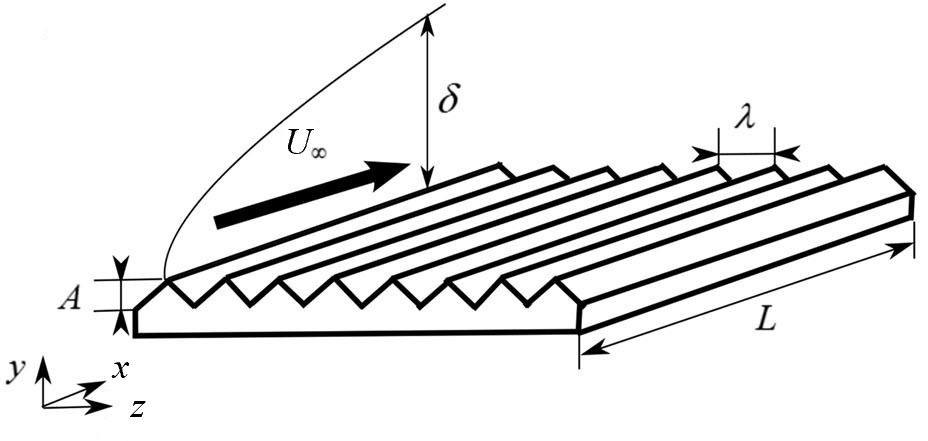
\includegraphics[width=0.5\linewidth]{introduction/fig/riblets.jpeg}
\caption{A schematic of triangular riblets the most commonly researched riblets. Figure modified from \cite{raayai-ardakani2019}.}
\label{fig:riblets}
\end{figure}

Therefore, researchers have begun to explore other ways to use passive flow control for turbulent \gls{dr}. The oblique \gls{ww} was first proposed by \textcite{chernyshenko2013} in 2013 to emulate the motions of in-plane spanwise wall oscillations in hopes that there will be a net energy decrease. We will devote the rest of this report discussing the merits of this curious passive flow control method.

%It is known that if in a turbulent flow the (wing) surface moves spanwise with a suitable velocity distribution, the friction drag is significantly reduced. Even though causing the wing surface to move requires energy input, the drag reduction is large enough to provide large energy savings. However, such motion is difficult to implement on an aircraft. In a paper (Chernyshenko, 2013, arxiv.org/abs/1304.4638) it was proposed to shape the rigid (not moving) surface in such a way that the resulting fluid motion will emulate the effect of the surface motion without the surface actually moving. For the case of the surface with sinusoidal waves at an angle to the mean flow direction, an optimisation of the angle and the height of the waves was performed. The later comparisons (Ghebali et al., 2017, aip.scitation.org/doi/10.1063/1.5003617) showed that the semi-empirical model of calculating the drag reduction used for optimisation was inaccurate. This might be due to this model not taking into account the energy dissipation due to the laminar viscosity and the shape of the mean velocity profile. This part of the dissipation is negligible at high Reynolds numbers, but it was significant at the Reynolds numbers studied. The project will consist in improving the semi-empirical model and repeating the shape optimisation using the improved model. It is recommended to see the first paper cited above to estimate the degree of mathematical proficiency needed for this project.

\section{Literature Review}
\subsection{The Spatial Stokes Layer (SSL)}%\label{ssec:ssl}
\subsubsection{Description}
The Stokes layer is one of the few known exact solutions to the Navier-Stokes equation describing the motion of a viscous fluid as a function of the wall normal coordinate $y$, whereby the infinitely long wall is located at the bottom at $y=0$ and oscillating harmonically in its own plane \cite{schlichting2016}. It turns out that the resulting oscillation in the fluid is only of significant magnitude very close to the wall in a so-called ``Stokes layer'' and is significantly damped outside of the said-layer.

\citeauthor*{jung1992} \cite{jung1992} were the first to suggest using a wall oscillating in the spanwise direction to reduce skin friction in 1992, exploiting the above phenomenon to obtain a maximum drag reduction of 40\% at a non-dimensional period of $T^+=100$ using \gls{dns}, a \gls{cfd} method \cite{karniadakis2003}. The $+$ superscript denotes non-dimensionalisation by wall units, which is based upon the wall friction velocity $\gls*{ut}=\sqrt{\frac{\gls*{tw}}{\gls*{ro}}}$, along with the kinematic viscosity $\gls*{nu}=\frac{\gls*{mu}}{\gls*{ro}},$ where \gls*{tw} is the wall shear stress of the fluid flow, \gls*{ro} is the density of the fluid, and \gls*{mu} is the dynamic viscosity of the fluid flow. The spanwise velocity of the wall is given by
\begin{equation}
	\gls*{spanwv} = \gls*{awall}\sin{\left( \frac{2\pi}{\gls*{per}}\gls*{tim} \right)}
,\end{equation}
where \gls*{awall} and \gls*{per} denotes the oscillation amplitude and period, and \gls*{tim} denotes time.
Moreover, when only one of the channel walls were oscillating, ``the reduction in turbulence activity was observed only near the oscillating wall, while the flow at the other wall remained fully turbulent'' \cite{jung1992}. When phase averaged this coincides with the Stokes layer with temporal forcing \cite{viotti2009}, we will therefore name it \gls{tsl}. \textcite{dhanak1999} observed that the duration of sweep events were reduced by 47\% and their strength reduced by 23\%, suggesting that the skin-friction reduction is a result of the ``attenuation in the formation of streamwise streaks \cite{karniadakis2003}.
%\textcite{karniadakis2003} provides an excellent review of research in in-plane wall motion up to 2003. 

As this is a form of active flow control, despite significant drag reductions, significant energy must also be expended to overcome the extra shear stress to create the spanwise motion of the fluid \cite{viotti2009}. \textcite{baron1996} was the first to consider the net energy savings from spanwise wall oscillation, and it is now accepted that the net energy savings is 10\% \cite{viotti2009, karniadakis2003}. However, this technique requires moving parts and therefore requires actuators, which is hard to implement in practical applications especially in transport applications.

\textcite{viotti2009} sought to extend the \gls{tsl} from a time-dependent forcing to a stationary, spatial forcing, which potentially allows an extension into passive solutions which can emulate the oscillation varying over space instead of time (such as the \gls{ww}). (------------------------------------------------------------------------------------------------------------------------------------------ kim and hussain--------------------------------???)
Letting $x$ be the streamwise coordinate, $y$ the wall-normal coordinate, and $z$ the spanwise coordinate, the spatial forcing law can be seen in Figure~\ref{fig:ssl}, and is given by
\begin{equation}
	\gls*{spanwv} = \gls*{awall}\sin{\left( \frac{2\pi}{\gls*{lm}_x} x \right)} 
,\end{equation}
where \gls*{awall} and $\gls*{lm}_x$ denotes the forcing amplitude and the forcing wavelength in the $x$ direction respectively. We will call this flow the \gls{ssl}.

\begin{figure}[htbp]
\centering
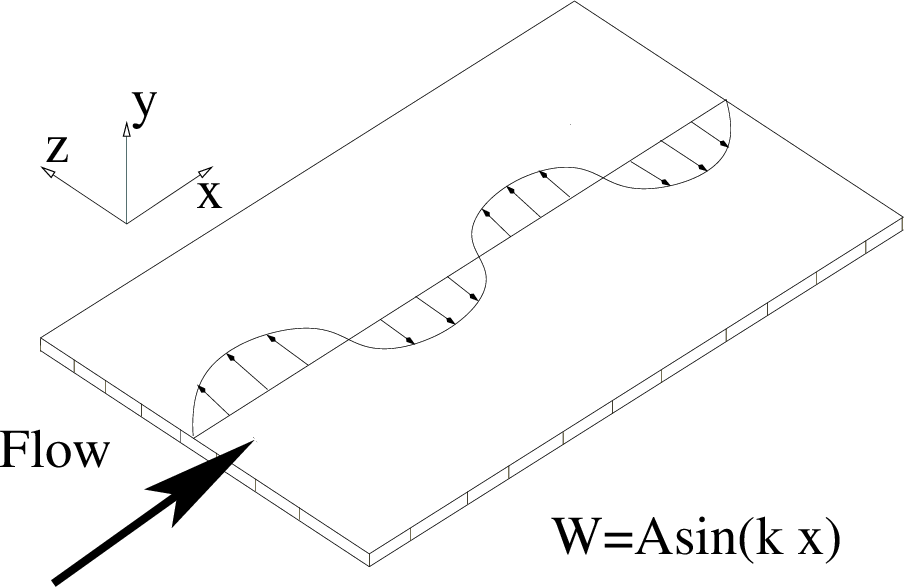
\includegraphics[width=0.5\linewidth]{introduction/fig/ssl.png}
\caption{Schematic of spanwise wall forcing from \cite{viotti2009}.}
\label{fig:ssl}
\end{figure}

\subsubsection{Solving for Velocity}
We will now analyse \gls{ssl} flow analytically following \textcite{chernyshenko2013}, who ultimately derives their analysis from \textcite{viotti2009}. We begin by solving for the velocity profile of \gls{ssl} flow by first defining the triple decomposition of velocity as follows
\begin{equation}
	\mathbf{U} = \overline{\mathbf{U} }+\tilde{\mathbf{u} }+\mathbf{u'}  
,\end{equation}
where $\overline{\mathbf{U} }$ is the velocity averaged over time, and space in the $x$ and  $z$ direction, $\tilde{\mathbf{u} }$ is the phase averaged velocity, and $\mathbf{u'} $ is the remaining stochastic turbulent part of the velocity. Unlike the traditional Reynolds decomposition, we have an extra phase dependent term, which is useful for periodic flows such as \gls{ssl} flow. We can adapt the definition given in \cite{baj2015} to our case and define for some phase angle $\gls*{phase}_0=\gls*{phase}(x_0+m \gls*{lm}_x,z_0+n \gls*{lm}_z)$,
\begin{equation}
	\tilde{\mathbf{u} }(y,\gls*{phase}_0):=\lim_{M\to\infty}\lim_{N\to\infty}\frac{1}{M}\frac{1}{N} \sum_{m=1}^{M} \sum_{n=1}^{N} \mathbf{U}(x_0+n \gls*{lm}_x,y,z_0 +m \gls*{lm}_z)-\overline{\mathbf{U} }(y)  
.\end{equation}
By including this average, we recognise that there will be periodicity in the $x$ component of the flow velocity; we also include periodicity in the $z$ component of the flow velocity since it will be useful for the \gls{ww} flow, and doesn't affect the definition for the \gls{ssl} flow, whose phase average has no $z$ dependence and therefore $\tilde{w}=0$.

With that definition, we can now solve for the phase averaged velocity of the \gls{ssl} flow. By linearising the \gls{bl} equations in the wall units of the flow around a linear profile, we ignore the stochastic fluctuations $\mathbf{u'} $ and let $\overline{\mathbf{U} }^{+} = (y^{+},0,0)$. Moreover, \gls{ssl} is time invariant. Thus, by analysing the order of various values as in \cite{schlichting2016}, and taking $\gls*{re}\to \infty$, we get
\begin{align}
	y^{+} \pdv{\tilde{u}^{+}}{x^{+}} + \tilde{v}^{+} &= -\pdv{p^{+}}{x^{+}} + \pdv[2]{\tilde{u}^{+}}{\left(y^{+}\right)} \label{eq:blx}\\
	0 &= -\pdv{p^{+}}{y^{+}}  \label{eq:bly}\\
	y^{+} \pdv{\tilde{w}^{+}}{x^{+}} &= -\pdv{p^{+}}{z^{+}} + \pdv[2]{\tilde{w}^{+}}{\left( y^{+} \right) } \label{eq:blz}\\
	0 &= \pdv{\tilde{u}^{+}}{x^{+}} +\pdv{\tilde{v}^{+}}{y^{+}} +\pdv{\tilde{w}^{+}}{z^{+}} \label{eq:blc}
,\end{align}
where $\gls*{press}^{+}$ is the non-dimensionalised pressure field. These are the general \gls{bl} equations (also known as \textit{Prandtl \gls{bl} equations}) when linearised around a linear mean profile (i.e. where we let $\overline{U}^{+}=(y^{+},0,0)$).

At the wall, we have $\tilde{u}\ssl\ps\rvert_{y\ps=0}=\tilde{v}\ssl\ps\rvert_{y\ps=0}=0$, and $\tilde{w}\ssl\ps\rvert_{y\ps=0}=\gls*{wht}\ps e^{i \gls*{wnum}_x\ps x\ps}$, where $\gls*{wht}\ps\ssl=A\ps$ is the wall oscillation amplitude, $\gls*{wnum}_x\ps = \frac{2\pi}{\lambda_x\ps}$ is the non-dimensional wavenumber, $i$ is the imaginary unit, the subscript $\gls*{sl}$ denotes that the variable is related to \gls{ssl} flow, and the superscript $+\gls*{sl}$ denotes non-dimensionalisation by the friction velocity specific to the \gls{ssl} flow $u_{\tau,\gls{sl}}=\sqrt{\frac{\tau_{w,\gls*{sl}}}{\gls*{ro}}} $. Although strictly speaking $\tilde{w}\ssl\ps\rvert_{y=0}$ is only the real part of the exponential function (as well as any other phase averaged terms that we prescribe the exponential function for the rest of this report), however analysis is much more easily done using the exponential function and only taking the real part thereof at the very end. Moreover, since the wall is flat, we expect the pressure gradient in all directions to be zero. We also only expect the spanwise periodic fluctuations to be non-zero, therefore $\tilde{u}\ssl=\tilde{v}\ssl=0  $. This means that to solve for $\tilde{w}\ps$ we only need Equation \eqref{eq:blz}.

Finally, we expect the spanwise velocity to vary not only in $x$ (due to the  $x$ dependence of the prescribed spanwise wall forcing), but also in  $y$ as the Stokes layer decreases in strength away from the wall. Therefore, we get $\tilde{w}\ps(x\ps,\check{y}\ps)=\gls*{wht}\ps\ssl\check{w}\ssl\ps e^{ik\ps_x x\ps}$, where we define $y^{+}=(k^{+}_x)^{-1 /3}\gls*{yck}$ in order to simplify or equations later, and $\check{w}\ssl \ps=\check{w}\ssl \ps(\check{y}\ps)$ as the only part of $\tilde{w}\ps$ dependent on $\check{y}\ps$.\glsadd{wck}
Therefore Equation \eqref{eq:blz} becomes
\begin{align}
	\left( k_x\ps \right) ^{-1 /3} \check{y}\ps \pdv{x\ps}(\hat{W}\ps \check{w}\ps\ssl e^{ik_x\ps x\ps})&= \pdv[2]{\left( (k_x\ps)^{-1 /3}\check{y} \right) }(\hat{W}\ps \check{w}\ps\ssl e^{ik_x\ps x\ps})\nonumber\\
	i \check{y}\ps \check{w}\ps\ssl &= \dv[2]{\check{w}\ps\ssl}{(\check{y}\ps)} 
.\end{align}
We can see that we can solve for $\check{w}\ps\ssl$ with only an \gls{ode}. We know that at the wall $\check{w}\ps\ssl\rvert_{\check{y}\ps=0}=1$, and since this is a Stokes layer, we want $\check{w}\ps\ssl \to 0$ as $\check{y}\ps\to \infty$. This \gls{ode} can either be solved numerically or be described by an Airy function (denoted $\Ai (\cdot)$) as follows,
 \begin{equation}
	 \check{w}\ps\ssl(\check{y}\ps)= \frac{\Ai(-i \check{y}\ps e ^{-\frac{4}{3}i\pi})}{\Ai(0)}
,\end{equation}
which gives
\begin{equation}
	w\ps\ssl = \Re \left[ \gls*{wht}\ps\ssl e^{i k_{x}\ps x}\frac{\Ai(-i \check{y}\ps e ^{-\frac{4}{3}i\pi})}{\Ai(0)}
 \right] 
.\end{equation}

\subsubsection{Net Power Saved}
Our ultimate goal is of course to find how much energy we might be able to save using \gls{ssl}. We will calculate the net power saved by having \gls{ssl} in both the top and bottom wall of an infinite flat channel (which was what was done in \textcite{viotti2009} such that comparisons can be made with \gls{dns}, which requires a finite domain), compared with a reference channel flow with no movement. We will denote variables relating to the reference flow with a subscript 0, and similar to the \gls{ssl} flow, we will denote non-dimensionalisation by the wall units of the reference flow with the superscript $+0$.

To find this elusive net power saving, we start with conservation of energy in the channel. Thus,
\begin{equation}
	P_\text{in}^{+}=P_\text{out}^{+}
,\end{equation}
where $P$ denotes power per unit area. We know for \gls{ssl}, $P_\text{in} $ includes some sort of external pump that powers the flow against drag (which we hope is reduced from the reference flow), as well as an actuator or motor which drives the oscillatory in-plane wall motion. Whereas for the reference flow $P_\text{in} $ does not have the latter. On the other hand, the $P_\text{out} $ of the system is purely through losses in heat, which comes from dissipation in the fluid, which, per unit area, is given by
\begin{equation}
	\Phi ^{+}=\int_{0}^{\infty} \overline{\left( \dv{\mathbf{U} \p}{y\p}  \right) ^2}  \dd{y\p} 
,\end{equation}
for one wall, where the overbar denotes conducting averaging and phase averaging in time and space in the $x,z$ directions. Despite this being channel flow, we integrate to infinity instead of the channel half height as the analysis is easier to deal with and it is presumed that $\dv{\mathbf{U}\p }{y\p} \to0$ quickly as $y\p\to\infty$ outside the boundary layer. Using the incredibly useful triple decomposition, the dissipation per unit area becomes
\begin{align}
	\Phi ^{+}&=\int_{0}^{\infty} \overline{\left( \dv{y\p}(\overline{\mathbf{U}} \p + \tilde{\mathbf{u} }\p + \mathbf{u'} )  \right) ^2}  \dd{y\p}\\ 
		 &=\int_{0}^{\infty} \left[ \overline{\left( \dv{\overline{\mathbf{U} }}{y\p}  \right) ^2}+\overline{\left( \dv{\tilde{\mathbf{u} }}{y\p}  \right) ^2} + \overline{\left(\dv{\mathbf{u'} }{y\p}\right) ^2} + 2\cancelto{0}{\left( \overline{\dv{ \overline{\mathbf{U} }}{y\p}\dv{ \tilde{\mathbf{u} }}{y\p} } + \overline{\dv{ \overline{\mathbf{U} }}{y\p}\dv{\mathbf{u'} }{y\p} } + \overline{\dv{ \tilde{\mathbf{u} }}{y\p}\dv{\mathbf{u'}}{y\p} } \right)}\phantom{--} \right] \dd{y\p} \label{eq:dissdisappear}  \\
		 &=\int_{0}^{\infty}  \overline{\left( \dv{\overline{\mathbf{U} }}{y\p}  \right) ^2}\dd{y\p}+\int_{0}^{\infty}  \overline{\left( \dv{\tilde{\mathbf{u} }}{y\p}  \right) ^2} \dd{y\p} + \int_{0}^{\infty}  \overline{\left(\dv{\mathbf{u'} }{y\p}\right) ^2} \dd{y\p}
.\end{align}
Wonderfully, the cross terms inside the final brackets of \ref{eq:dissdisappear} all go to zero since the overbar for dissipation involves both the mean averaging and phase averaging, and since $\overline{\overline{a}b}=\overline{a}\overline{b}$ for any $a,b$, and the average of a fluctuating quantity is zero.
Moreover, since the flows being considered throughout the rest of the report have a mean velocity in the $y$ or $z$ direction, nor will they have a phase averaged velocity in the $y$ direction we can then reduce the dissipation further to 
\begin{align}
	\Phi \p &=\int_{0}^{\infty}  \overline{\left( \dv{\overline{U}}{y\p}  \right) ^2}\dd{y\p}+\int_{0}^{\infty}  \overline{\left( \dv{y\p}(\tilde{u},\tilde{w},0)  \right) ^2} \dd{y\p} + \int_{0}^{\infty}  \overline{\left(\dv{\mathbf{u'} }{y\p}\right) ^2} \dd{y\p}\\
	&=\int_{0}^{\infty}  \overline{\left( \dv{\overline{U}}{y\p}  \right) ^2}\dd{y\p}+\int_{0}^{\infty}  \overline{\left( \dv{\tilde{u}}{y\p}  \right) ^2} \dd{y\p} +\int_{0}^{\infty}  \overline{\left( \dv{\tilde{w}}{y\p}  \right) ^2} \dd{y\p} + \int_{0}^{\infty}  \overline{\left(\dv{\mathbf{u'} }{y\p}\right) ^2} \dd{y\p}\\
	&= \Phi_{\overline{U}}\p + \Phi _{\tilde{u}}\p + \Phi _{\tilde{w}}\p + \Phi _{\mathbf{u'} }\p
.\end{align}
For the reference flow $\Phi _{0}\pz=\Phi _{\overline{U},0}\pz+\Phi _{\mathbf{u'} ,0}\pz$, whereas for the \gls{ssl} flow $\Phi \ssl\ps=\Phi _{\overline{U},\gls*{sl}}\ps + \Phi _{\tilde{w},\gls*{sl}}\ps + \Phi _{\mathbf{u'},\gls*{sl} }\ps$. Therefore we can call the $\overline{U}$ and $\mathbf{u'} $ portions of dissipation drag, and the extra $\tilde{w}$ portion of dissipation an extra required portion for the \gls{ssl} flow. We define

%, we can determine this as a function of the amount of power saved (i.e. the \gls{dr}) and the amount of power used to effect the oscillatory forcing. To begin 

\subsection{The Oblique Wavy Wall (WW)}
\subsubsection{Description}
As mentioned in Section \ref{sec:motivation}, \gls{ssl} is

%Intro: Motivation, Riblets, and others in general, Lit Review – Stokes Layer Results; SSL+Chernyshenko. Refer to Ghebali DNS. End:Formulation of problem: want to be able to predict drag reduction by WW as f’n of $k_x, k_z$, and What



%It is known that if in a turbulent flow the (wing) surface moves spanwise with a suitable velocity distribution, the friction drag is significantly reduced. Even though causing the wing surface to move requires energy input, the drag reduction is large enough to provide large energy savings. However, such motion is difficult to implement on an aircraft. In a paper (Chernyshenko, 2013, arxiv.org/abs/1304.4638) it was proposed to shape the rigid (not moving) surface in such a way that the resulting fluid motion will emulate the effect of the surface motion without the surface actually moving. For the case of the surface with sinusoidal waves at an angle to the mean flow direction, an optimisation of the angle and the height of the waves was performed. The later comparisons (Ghebali et al., 2017, aip.scitation.org/doi/10.1063/1.5003617) showed that the semi-empirical model of calculating the drag reduction used for optimisation was inaccurate. This might be due to this model not taking into account the energy dissipation due to the laminar viscosity and the shape of the mean velocity profile. This part of the dissipation is negligible at high Reynolds numbers, but it was significant at the Reynolds numbers studied. The project will consist in improving the semi-empirical model and repeating the shape optimisation using the improved model. It is recommended to see the first paper cited above to estimate the degree of mathematical proficiency needed for this project.


%This is one of the most important components of the dissertation. It should begin with a clear statement of what the project is about so that the nature and scope of the project can be understood by a lay reader. It should summarise everything you set out to achieve, provide a clear summary of the project's background and relevance to other work and give pointers to the remaining sections of the dissertation which contain the bulk of the technical material.
%
%Further information can be found here: \url{https://goo.gl/k2huN9}.
%
%\section{\LaTeX{} code examples and formatting tips}
%Hello, here's a citation \cite{greenwade93}. References are stored in a Bibtex file. Google Scholar and IEEExplore allow you to download citations of papers in Bibtex format from their search engine. Some people use JabRef (\url{http://www.jabref.org}) to manage their database of references.
%
%This is an inline equation $\Gamma(t)=K_i e^{\sin^2(\omega_t)}$. The first paragraph appears without indent but the following ones will have an indentation.
%
%This is an actual named equation:
%\begin{equation}
%v(x)=\frac{1}{2}\sin(2 \omega t + \phi) e^{-j s t}
%\label{eq:cacona}
%\end{equation}
%\noindent where $\omega$ is the angular speed. Notice that symbols liks $\omega$ should be written in italics whereas measurement units such as V for Volts appear as normal text. This paragraph didn't have an indentation because the first sentence was linked to the definition of equation (\ref{eq:cacona}). A code snippet for an example program is shown in Listing~\ref{lst:code1}.
%
%\begin{lstlisting}[caption=Source code for {\it hello.m},label=lst:code1,breaklines=true,basewidth=4pt,prebreak=**,postbreak=**,frame=single]
%for i:=maxint to 0 do
%begin
%{ do nothing }
%end;
%Write('Case insensitive ');
%Write('Pascal keywords.');
%\end{lstlisting}
%
%The characteristic parameters of the system are sumarised in Table~\ref{tab:tab1}. A figure is shown Fig~\ref{fig:felix}, we don't necessarily know if this figure will appear below, above or elsewhere; therefore, the text should never refer to the figure with sentences such as {\it "As shown here:"}.
%%
%\begin{figure}[htbp]
%\centering
%
\includegraphics[width=0.3\linewidth]{introduction/fig/Felix_the_cat.pdf}
%\caption{Felix the Cat}
%\label{fig:felix}
%\end{figure}
%
%\begin{table}[htbp]
%	\centering
%	\begin{tabular}{lll}
%		Parameter & Value & Units\\
%		\hline
%		$P$ & 1 & kW \\
%		$Q$ & 0 & kVAr\\
%	    \hline
%	\end{tabular}
%	\caption{Characteristic parameters of the system}
%	\label{tab:tab1}
%\end{table}
%
%\begin{samepage}
%Sometimes, the symbols in an equation are defined as follows\footnote{Some authors like to define their symbols this way.}:
%\begin{equation}
%	V(t)=A \sin(\omega t+\theta_0)
%\end{equation}
%\begin{tabular}{lll}
%	where & $V$ & is a voltage waveform,\\
%	& $A$ & is the amplitude of the voltage,\\
%	& $\omega$ & is the angular frequency,\\
%	& $t$ & is the time.
%\end{tabular}
%\end{samepage}
%
%\subsection{A brief comparison between a proper plot and a horrible plot}
%
%Figure \ref{fig:fig2} contains two plots of the same waveform. Subfigure \ref{fig:fig2sub1} shows a badly formatted figure, Subfigure \ref{fig:fig2sub2} shows a much better formatted figure. The problems with Subfigure \ref{fig:fig2sub1}, listed by order or relevance, are the following:
%
%\begin{enumerate}
%    \item The font size is too small to be read properly.
%    \item The axes aren't labeled properly: the horizontal axis is not labeled and the units of the vertical axis are unknown. Further, symbols must be written in italics whereas numbers and units must be written as normal text.
%    \item The choice of limits for the axes is not good, the figure has wide useless empty spaces. The most relevant part of the waveform is the transient that happens between times $t=$0 and $t=$0.05 s, which is less than 10\% of the timespan shown in the figure.
%    \item The figure has been scaled without keeping the original aspect ratio and fonts look narrower than they would if the figure had been scaled properly.
%    \item The plot doesn't have grid lines. This makes it hard to read the exact value (ie time, voltage) of points in the trace.
%    \item The width of the trace is too thin and may not be visible if printed in low resolution.
%    \item The choice of units of the vertical axis aren't the best. For example, in this case the plot would be easier to read if voltage had been expressed in kV instead of V.
%    \item The figure was exported as a bitmap (e.g. png, jpg, bmp) instead of being exported in vector format (e.g. eps, svg, pdf) and visual artifacts appear when the figure is scaled up or down in order to fit in the document.
%\end{enumerate}
%
%\begin{figure}[htbp]
%	\centering
%	\subfigure[A horrible one.]{
%		\label{fig:fig2sub1}
%        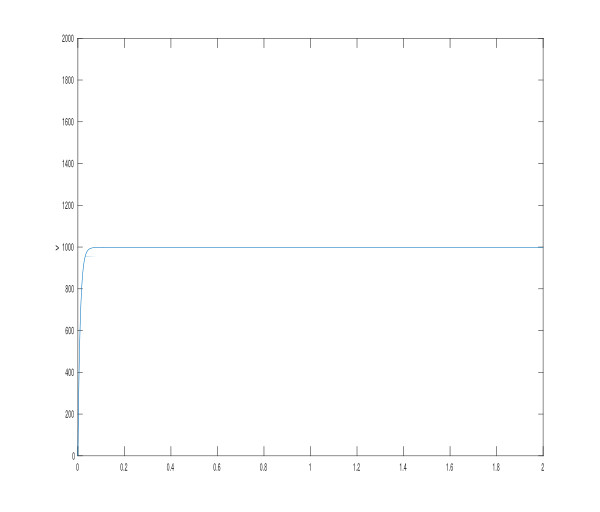
\includegraphics[width=0.5\linewidth]{introduction/fig/figure1.jpg}}
%	\subfigure[A proper one.]{
%		\label{fig:fig2sub2}
%		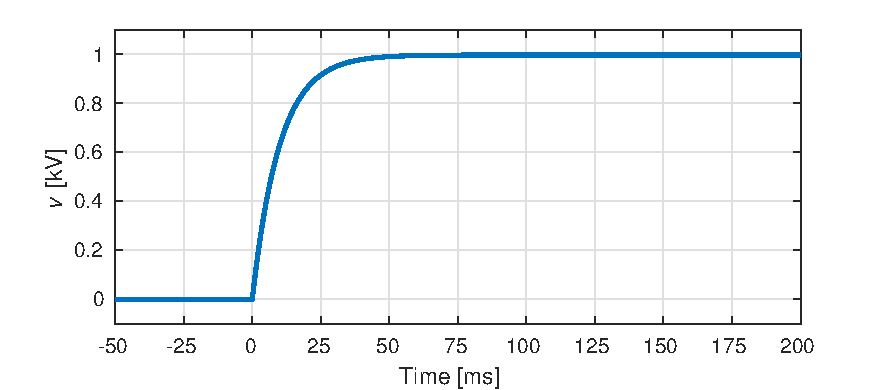
\includegraphics[width=0.6\linewidth]{introduction/fig/figure2.pdf}}
%	\caption{A figure with two subfigures.}
%	\label{fig:fig2}
%\end{figure}
%
%\begin{landscape}
%	\begin{figure}[htbp]
%\centering
%
\includegraphics[width=0.5\linewidth]{introduction/fig/Felix_the_cat.pdf}
%\caption{Here's a large drawing of Felix the Cat that wouldn't fit in a portrait page}
%\label{fig:felix2}
%\end{figure}
%\end{landscape}
%
%\section{Objectives}
%\section{Challenges}
%\section{Contributions}

%\chapter{Background}
The background section of the dissertation should set the project into context by relating it to existing published work which you read at the start of the project when your approach and methods were being considered. There are usually many ways of solving a given problem, and you shouldn't just pick one at random. Describe and evaluate as many alternative approaches as possible. The background section is often included as part of the introduction but can be a separate chapter if the project involved an extensive amount of research.

The published work may be in the form of research papers, articles, text books, technical manuals, or even existing software or hardware of which you have had hands-on experience. Don't be afraid to acknowledge the sources of your inspiration; you are expected to have seen and thought about other people's ideas; your contribution will be putting them into practice in some other context. However, you must avoid plagiarism: if you take another person's work as your own and do not cite your sources of information/inspiration you are being dishonest; in other words you are cheating.
\chapter{Project - Wavy Wall Analysis}\glsresetall
\section{Power Saved by the Wavy Wall (WW)}
With our definition of $P_\text{sav,\gls*{wv}}$ staying the same, we no longer believe it is equal to $P_\text{sav,\gls*{sl}}$. However, since we matched the periodic spanwise shear, we still maintain that the reduction in stochastic turbulent dissipation is the same between the \gls{ww} and \gls{ssl} flow, i.e. $\frac{\Delta \Phi _{\mathbf{u} ',\gls*{sl}}\pz}{\Phi _{0}\pz}=\frac{\Delta \Phi _{\mathbf{u} ',\gls*{wv}}\pz}{\Phi _{0}\pz}$. Therefore,
\begin{align}
	P_\text{sav,\gls*{wv}}	-P_\text{sav,\gls*{sl}} &= 100\%\frac{\Delta \Phi _{\overline{U },\gls*{wv}}\pz+\Delta \Phi _{\mathbf{u} ',\gls*{wv}}\pz}{\Phi \zz\pz}-100\% \frac{\Delta \Phi _{\overline{U },\gls*{sl}}\pz+\Delta \Phi _{\mathbf{u} ',\gls*{sl}}\pz}{\Phi \zz\pz}\\
	P_\text{sav,\gls*{wv}}	-P_\text{sav,\gls*{sl}}  &= 100\% \frac{\Delta \Phi _{\overline{U },\gls*{wv}}\pz-\Delta \Phi _{\overline{U },\gls*{sl}}\pz}{\Phi \zz\pz}\\
	P_\text{sav,\gls*{wv}} &= 100\% \frac{ \Phi _{\overline{U },\gls*{wv}}\pz-\Phi _{\overline{U },\gls*{sl}}\pz}{\Phi \zz\pz}+P_\text{sav,\gls*{sl}}
.\end{align}


\section{The Spatial Stokes Layer (SSL) Mean Velocity Profile}\label{sec:sslmean}
Since we do not know the shape of the \gls{ww} mean streamwise velocity profile to figure out dissipation due to the mean profile, we must start elsewhere. The \gls{ssl} mean streamwise velocity profile $\overline{U}\ssl\ps$ was given by \vqt, along with that of \gls{tsl}, the reference channel flow, and $\overline{U}^{+}=y^{+}$ for comparison (Figure~\ref{fig:sslmeanprofile}). We can see that at $y^{+}<10$, they all coincide to the linear profile $\overline{U}^{+}=y^{+}$, and at some point between $10<y^{+}<40$, they stop being curved on the logarithmic plot and become straight with similar slopes, indicating a logarithmic profile at higher $y^{+}$. In fact, like other \gls{dr} techniques (e.g. riblets), the \gls{dr} is noticeable as a thickening of the viscous sublayer causing an upward shift in this logarithmic portion of the mean velocity profile \cite{viotti2009,choi1989,luchini1996}. 

\begin{figure}[htbp]
	\centering
	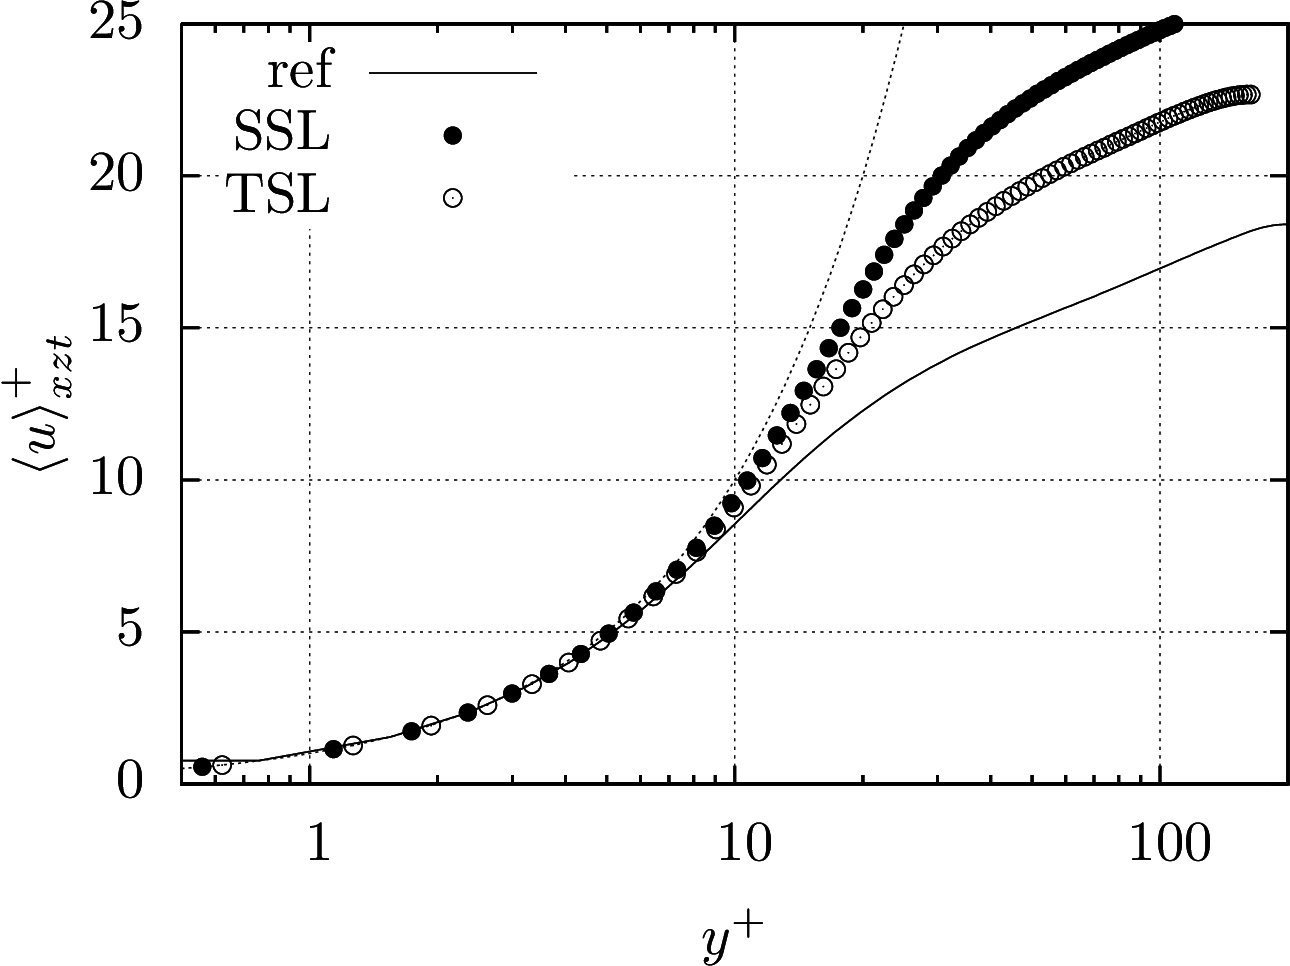
\includegraphics[width=0.7\linewidth]{project/fig/sslmeanprofile.png}
	\caption[Streamwise mean velocity profiles of SSL and reference flow]{Streamwise mean velocity profiles in wall units averaged in $x$-$z$ space, time, and phase ($\overline{U}^{+}\equiv \left<u \right>^{+}_{xzt}$) for \gls{ssl}, \gls{tsl}, the reference flow, and $\overline{U}^{+}=y^{+}$ (dotted line) for comparison \cite{viotti2009}.}
	\label{fig:sslmeanprofile}
\end{figure}

In order to see the differences more clearly, the  \gls{ssl} and refence flow data from Figure~\ref{fig:sslmeanprofile} were digitised using the web app webplotdigitiser. Then a curve fit was implemented and plotted in Figure~\ref{fig:sslmpcf} using an analytical fit for a turbulent plane channel flows given in an unpublished supplement to \cite{chernyshenko2021}. Abnormally, though, when the curve fit given for the mean streamwise velocity was used, the derivative thereof fluctuated much more than expected. Therefore, the curve fit for the second moments of velocity near the wall (root mean square velocity) was trialled instead, which produced much more reasonable derivative whilst also maintaining a good curve fit in and of itself. This latter curve fit is given as
\begin{equation}
	y^{+}  \frac{a\left(y^{+}\right)^2 + by^{+} + c}{q\left(y^{+}\right)^2 + ry^{+} + 1} + p \left( \ln(y^{+}+15)-\ln(15)\right)\label{eq:curvefit}
,\end{equation}
where $a,b,c,p,q,r$ are some coefficients. This function, however, does not guarantee that $\dv{U^{+}}{y^{+}} =1$ at the wall, which would be most accurate. We can see again that at $y^{+}<10$, the curves both fit on the $\overline{U}^{+}=y^{+}$ line. Then there is an area where the two curves diverge, but then, at around $y^{+}>60$, the gradients $\dv{\overline{U}^{+}}{y^{+}} $ seem to look fairly similar and in fact become negligible. This, as \textcite{viotti2009} had done, lead us to conjecture that the logarithmic portion of the \gls{ssl} mean velocity profile was the same as that of the reference flow but with an extra vertical shift.

Therefore, we take the well known logarithmic portion of the law of the wall, which applies to the reference flow,
\begin{equation} 
	\overline{U}\pz\zz=\frac{1}{\kappa}\ln y\pz+B\label{eq:cfref}
,\end{equation}
where $\kappa=0.41$, and  $B=5.0$ \cite{schlichting2016}, and add a vertical shift  $\Delta h$ to get
 \begin{equation}
	 \overline{U}\ps\ssl=\frac{1}{\kappa}\ln y\ps +B+\Delta h\ssl\label{eq:cfww}
.\end{equation}
$\Delta h$ can easily be estimated by drawing a straight line that follows the logarithmic portion of the \gls{ssl} mean profile (where $y^{+}>60$ ) on the logarithmic scale (in Figure~\ref{fig:sslmeanprofile}), reading the intercept of said straight line, and subtracting by $B$. By this method it was found that  $\Delta h\approx8$. Curve fits using Equations~\eqref{eq:cfref} and \eqref{eq:cfww} are plotted in Figure~\ref{fig:sslmpest}.

\begin{figure}[htbp]
	\centering
	\subfigure[Curve fits.]{
		\label{fig:sslmpcf}
        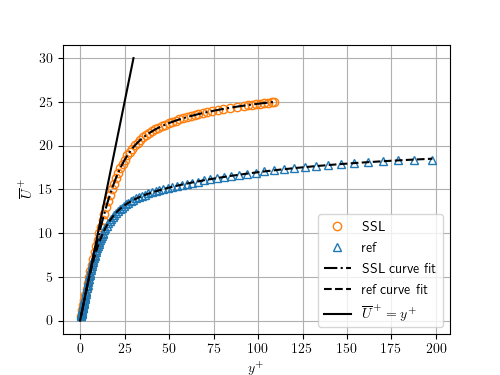
\includegraphics[width=0.485\linewidth]{project/fig/sslmeanprofilelin.png}}
	\subfigure[Estimated logarithmic profiles.]{
		\label{fig:sslmpest}
		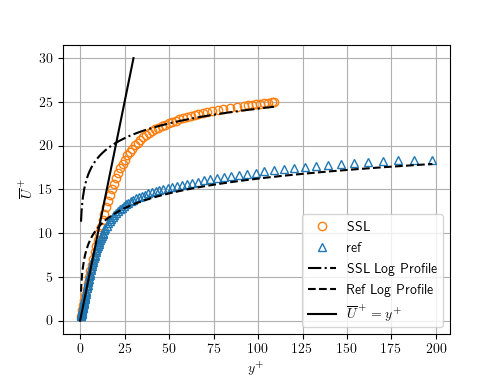
\includegraphics[width=0.485\linewidth]{project/fig/sslmeanprofileest.png}}
		\caption[Mean streamwise velocity profiles of SSL and reference flows, and analytical approximations thereof]{Both plots show data on the mean streamwise velocity profiles of \gls{ssl} (orange-circle) and the reference flow (blue-triangles) which were digitised from \textcite{viotti2009} (shown in Figure~\ref{fig:sslmeanprofile} and plotted on a linear scale, as well as $\overline{U}^+=y^+$ (solid-line). }
	\label{fig:sslmplin}
\end{figure}
The validity of using the same logarithmic profile with vertical shift as an estimate can be further seen in Figure~\ref{fig:sslmpdiff}, where the squares of the derivatives of the curvefits found using Equation~\eqref{eq:curvefit} were plotted for the \gls{ssl} and reference flows. We can see that the differences in the derivatives are negligibly small. Moreover, since dissipation is equal to the integral of this derivative from 0 to infinity, we can see that contributions at $y^{+}>60$ are negligible. Whilst we can only numerically integrate the curve fitted solution, we can actually analytically integrate the estimated solution as
\begin{align}
	\Phi _{\overline{U}}^{+} &= \int_{0}^{y_{\times}^{+}} \left| \frac{dy^{+}}{dy^{+}} \right|^2dy^{+} + \int_{y_{\times}^{+}}^{\infty} \left| \frac{d\left( \frac{1}{\kappa}\ln y^{+} +B+\Delta h\right) }{dy^{+}} \right|^2dy^{+}  \\
	&= \int_{0}^{y_{\times}^{+}} 1dy^{+} + \frac{1}{\kappa^2}\int_{y_{\times}^{+}}^{\infty} \left| \frac{1}{y^{+}} \right|^2dy^{+}  \\
	&= y_{\times}^{+} + \frac{1}{\kappa^2}\frac{1}{y_{\times}^{+}}\\
	&=\frac{\left(  \kappa y_{\times}^{+}  \right) ^2+ 1}{\kappa^2 y_{\times}^{+}}\label{eq:fiycross}
,\end{align}
where \gls*{ycrs} is the single point at which the linear profile crosses the logarithmic profile. For \gls{ssl}, we have We find that for this estimated profile, the ratio $\frac{\Phi _{\overline{U},\gls*{sl}}\ps}{\Phi _{\overline{U},\gls*{zer}}\pz}\rvert_\text{est}=1.818$, whereas the same ratio for the curve fitted profile $\frac{\Phi _{\overline{U},\gls*{sl}}\ps}{\Phi _{\overline{U},\gls*{zer}}\pz}\rvert_\text{cfit}=1.650$. The estimated ratio is only 10.1\% higher than that of the curve fitted solution. Therefore, the idea is that perhaps if we could model the mean profile of the \gls{ww} using the linear plus logarithmic profile approach, perhaps it would be good enough to measure the net power reduction of the \gls{ww} flow.
\begin{figure}[htbp]
	\centering
	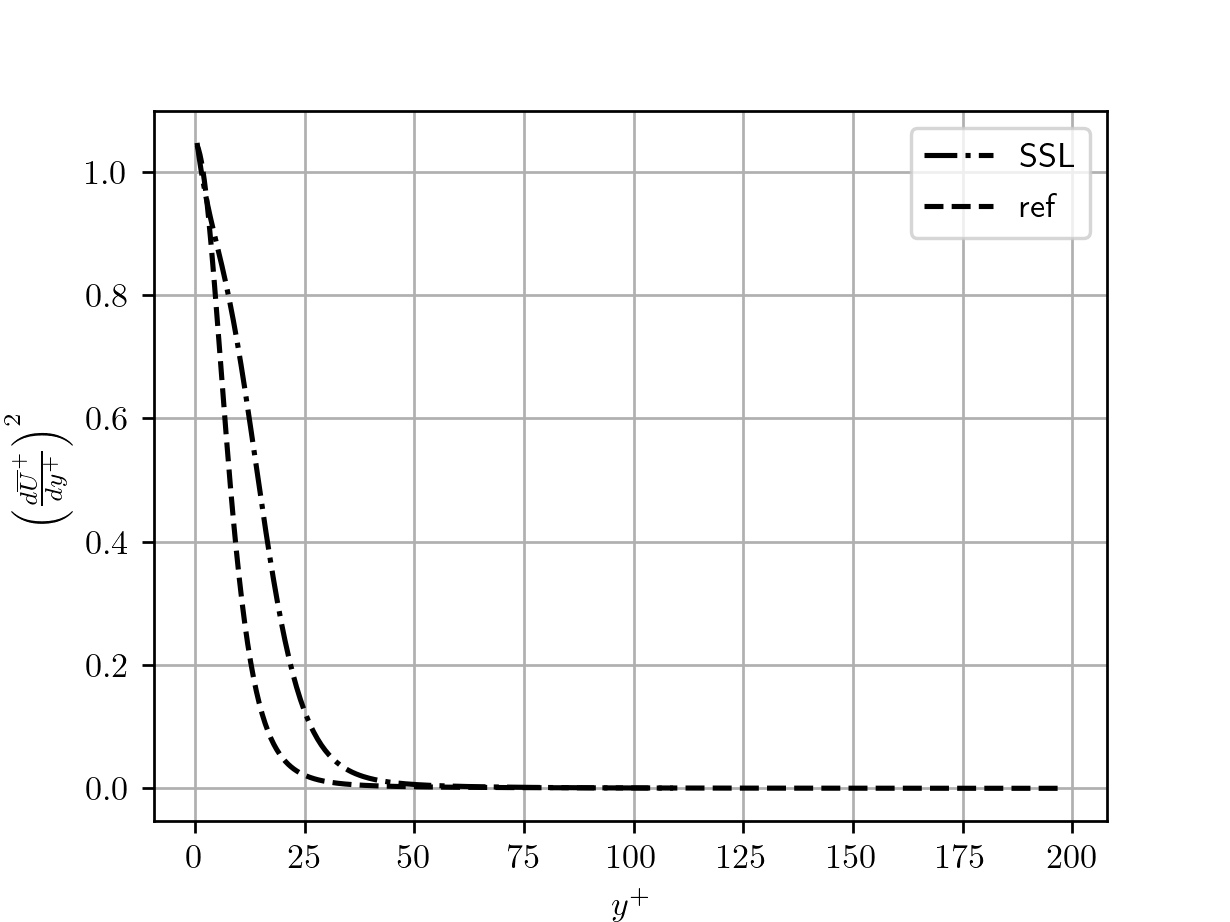
\includegraphics[width=0.7\linewidth]{project/fig/sslmeandiff.png}
	\caption[Mean streamwise shear profile squared of SSL and reference flows]{The squared mean streamwise shear profiles of \gls{ssl} (dot-dash), and reference (dash) flows, i.e. the squared derivative of mean streamwise velocity profiles $\dv{\overline{U}^{+}}{y^{+}} $ obtained using Equation~\eqref{eq:curvefit} for $\overline{U}^{+}$, which is shown in Figure~\ref{fig:sslmpcf}.}
	\label{fig:sslmpdiff}
\end{figure}

\section{Modelling the Wavy Wall (WW) Mean Velocity Profile}
With Equation~\eqref{eq:cfww}, \textcite{luchini1996} wrote that ``an increment in [$B$ i.e.  $\Delta h$] can be quantitatively translated into drag reduction because [$B$ ] appears explicitly in the drag formulae that'' since we can just integrate the mean velocity profile. For a turbulent boundary layer over a flat plate, the friction formula is given by
\begin{equation}
	\left( \frac{C_f}{2} \right) ^{-1 /2} = \frac{1}{\kappa}\ln \left[ \left( \frac{C_f}{2} \right) ^{1 /2 } \Rey_D \right] + 2.2 + B
,\end{equation}
where $\Rey_D $ is based on the velocity boundary-layer thickness \cite{white1991}. It turns out that for small increments in $B$,
 \begin{equation}
	 \frac{\Delta C_f}{C_{f,\gls*{zer}}}=-\frac{\Delta h}{\left(2C_{f,\gls*{zer}}\right)^{-1 /2} +\kappa /2}
,\end{equation}
where $\Delta C_f=C_f-C_{f,\gls*{zer}}$ \cite{luchini1996}. For \gls{ww}, $P_\text{net,\gls*{wv}} \equiv100\% \frac{C_{f,\gls*{zer}-C_{f,\gls*{wv}}}}{C_{f,\gls*{zer}}}$. Therefore,
\begin{align}
	-\frac{P_\text{net,\gls*{wv}}}{100\%} &=-\frac{\Delta h\ww}{(2C_{f,\gls*{zer}})^{-1 / 2}+\kappa / 2}\\
	\Delta h\ww &= \frac{P_\text{net,\gls*{wv}}}{100\%\left[(2C_{f,\gls*{zer}})^{-1 / 2}+\kappa / 2\right]}
.\end{align}
Thus, we believe the \gls{ww} mean velocity profile can be modelled by
\begin{equation}
	\overline{U}\ww\pw =
	\begin{cases}
		y\pw, & y\pw\leq y_{\times}\pw\\
		\frac{1}{\kappa}\ln y\pw +B +\frac{P_\text{net,\gls*{wv}}}{100\%\left[(2C_{f,\gls*{zer}})^{-1 / 2}+\kappa / 2\right]}, & y\pw>y_{\times}\pw
	\end{cases}
.\end{equation}

By modelling the \gls{ww} mean velocity profile like so, we can find $P_\text{net,\gls*{wv}} $ as only a function of $y_{\times}\pw$ by solving the two cases as a system of equations, i.e. we let $\overline{U}\ww\pw=y\pw$ in the logarithmic profile as follows
\begin{align}
	\overline{U}\pw\ww &=\frac{1}{\kappa}\ln y\pw +B +\frac{P_\text{net,\gls*{wv}}}{100\%\left[(2C_{f,\gls*{zer}})^{-1 / 2}+\kappa / 2\right]} \\
	y_\times\pw &=\frac{1}{\kappa}\ln y_\times\pw +B +\frac{P_\text{net,\gls*{wv}}}{100\%\left[(2C_{f,\gls*{zer}})^{-1 / 2}+\kappa / 2\right]} \\
	P_\text{net,\gls*{wv}} &=100\left(  y_{\times}\pw - \frac{1}{\kappa}\ln y_{\times}\pw - A \right) \left( (2C_{f,0})^{-\frac{1}{2}} +\frac{\kappa}{2} \right) 
.\end{align}

Moreover, we can also employ Equation~\eqref{eq:fiycross} combined with the wall unit conversions just as Equation~\eqref{eq:fislconv} to get
\begin{equation}
	\Phi _{\overline{U},\gls*{wv}}\pz = \Phi _{\overline{U},\gls*{wv}}\pw \left( \frac{\tau_{w,\gls*{wv}}}{\tau_{w,\gls*{zer}}} \right) ^{3 /2 }=\frac{\left(  \kappa y_{\times}^{+}  \right) ^2+ 1}{\kappa^2 y_{\times}^{+}} \left(  \frac{\tau_{w,\gls*{wv}}}{\tau_{w,\gls*{zer}}} \right) ^{3 /2 } \label{eq:fiwwpzycr}
.\end{equation}

But there is a slight problem here. Previously, for $\frac{\tau_{w,\gls*{sl}}}{\tau_{w,\gls*{zer}}}$, we have simply said this is equal to $1-\frac{P_\text{sav,\gls*{sl}}}{100\%} $ in an \gls{ssl} flow. However, in a \gls{ww} flow, this is not necessarily the case. $\tau_w$ only involves the frictional drag of the flow (the wall shear stress), but leaves out pressure drag which is present in the  \gls{ww} due to the undulations which create pressure gradients. As of writing, the author knows of no way to extract $\frac{\tau_{w,\gls*{wv}}}{\tau_{w,\gls*{zer}}}$. The only solution was to turn to \gls{dns} by \sgt. Through their results we were able to find that although the drag reduction and pressure drag reduction were of the same order, the pressure drag reduction was at least an order of magnitude smaller than the total drag, i.e. we conjecture that pressure drag on the \gls{ww} is $\ll \tau_{w,\gls*{wv}}$. Therefore, we let
\begin{equation}
	P_\text{net,\gls*{wv}}\approx 100\% \frac{\tau_{w,\gls*{zer}-\tau_{w,\gls*{wv}}}}{\tau_{w,\gls*{zer}}} \implies  \frac{\tau_{w,\gls*{wv}}}{\tau_{w,\gls*{zer}}}\approx1-\frac{P_\text{net,\gls*{wv}} }{100\%}\label{eq:tauassump}
,\end{equation}
even though it isn't necessarily true.

\section{Net Power Reduction by Wavy Wall (WW) - Results}
By accepting the assumption in Equation~\eqref{eq:tauassump}, quite accidentally, we have now stumbled upon a closed set of equations for which we can solve numerically for a given  $\lambda_x\pz$, $\lambda_z\pz$, and $\hat{W}\ssl\pz$. We start by recognising that nowhere in our analysis did we need to involve $P_\text{req,\gls*{wv}}=r_\text{min} P_\text{req,\gls*{sl}}  $. Therefore, $r_\text{min} $ stays the same, and $\frac{\lambda_x\pz}{\lambda_z\pz}\rvert_\text{opt} $ stays the same. Thus the closed set of equations is as follows
\begin{align}
	P_\text{net,\gls*{wv}} &= P_\text{sav,\gls*{wv}} + r_\text{min} P_\text{req,\gls*{sl}} \label{eq:Pnetww}\\  
	P_\text{sav,\gls*{wv}} &=  100\% \sqrt{\frac{C_{f,\gls*{zer}}}{2}}\left(  \frac{\left(  \kappa y_{\times,\gls*{wv}}\pw  \right) ^2+ 1}{\kappa^2 y_{\times,\gls*{wv}}\pw} \left( \frac{\tau_{w,\gls*{wv}}}{\tau_{w,\gls*{zer}}} \right) ^{\frac{3}{2}}-\Phi _{\overline{U},\gls*{sl}}\pz\right) +P_\text{sav,\gls*{sl}} \label{eq:Psavww}\\
	P_\text{net,\gls*{wv}} &=100\%\left(  y_{\times}\pw - \frac{1}{\kappa}\ln y_{\times}\pw- B \right) \left( (2C_{f,0})^{-\frac{1}{2}} +\frac{\kappa}{2} \right) \label{eq:ycross}\\
	P_\text{req,\gls*{sl}} &= -100\%\left( \hat{W}\pz  \right) ^2\sqrt{\frac{C_{f,\gls*{zer}}}{2}}   \left( \frac{2\pi (1-P_\text{sav,\gls*{sl}} / 100\%) }{\lambda_x\pz}\right) ^{\frac{1}{3}}\int_{0}^{\infty} \frac{1}{2} \left| \frac{d\check{w}\ps\ssl}{d\check{y}\ps} \right| ^2 d\check{y}\ps \\ 
		P_\text{sav,\gls*{sl}} &= f\left(\lambda_x\pz, \hat{W}\ssl\pz\right) \text{ (from Equation~\eqref{eq:psavsl})}\\
		\Phi _{\overline{U},\gls*{sl}}\pz &= \left( 1-\frac{P_\text{sav,\gls*{sl}} }{100\%} \right)  \left[\frac{\left(  \kappa y_{\times,\gls*{sl}}\ps  \right) ^2+ 1}{\kappa^2 y_{\times,\gls*{sl}}\ps}\right]\\
	y_{\times,\gls*{sl}}\ps&=\frac{1}{\kappa}\ln  y_{\times,\gls*{sl}}\ps +B+\Delta h\ssl \\
	C_{f,\gls*{zer}} &= 0.00336\Rey_{\tau}^{-0.273}
,\end{align}
where $\Delta h \ssl=8$, $\Rey_{\tau} = 200$,  $\kappa=0.41$,  $B=5.0$,  $r_\text{min} =5.846$, and $\int_{0}^{\infty} \frac{1}{2} \left| \frac{d\check{w}\ps\ssl}{d\check{y}\ps} \right| ^2 d\check{y}\ps = 0.3157$.

We solved this for $P_\text{net,\gls*{wv}} $ as a function of $\lambda_x\pz$ for $\hat{W}\ssl\pz=1,2,6,12$ and plotted them in Figure~\ref{fig:pnetww}. The code for solving these equations, as well as others in this report, along with many of the figures generated is in Appendix~\ref{app:code}.
\begin{figure}[htbp]
	\centering
	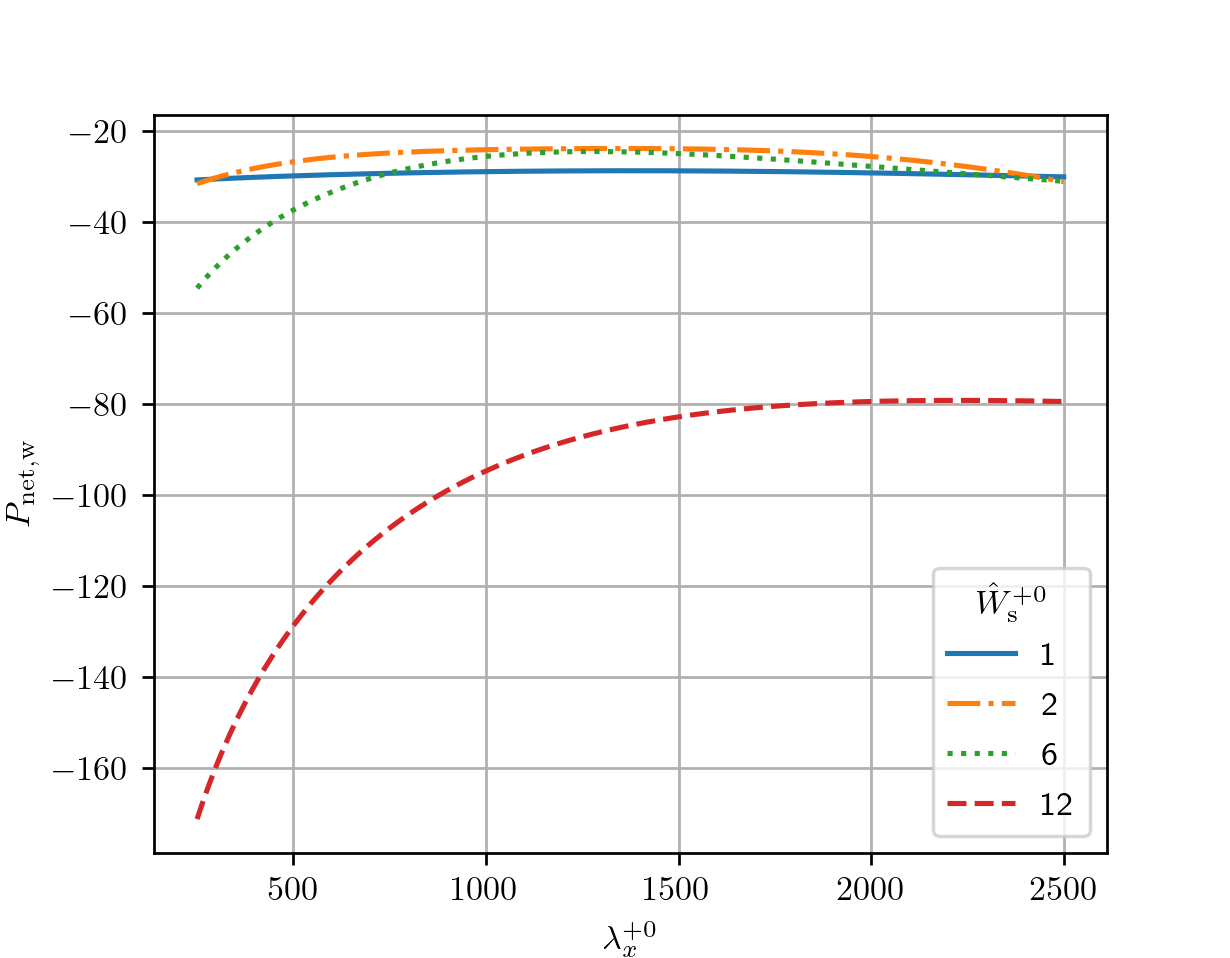
\includegraphics[width=0.7\linewidth]{project/fig/pnetww.png}
	\caption[Net power reduction for the wavy wall $P_\text{net,w}$]{Calculated net power reduction $P_\text{net,\gls*{wv}} $ for the wavy wall $P_\text{net,\gls*{wv}} $.}
	\label{fig:pnetww}
\end{figure}

%\chapter{Evaluation}
\chapter{Conclusion}\glsresetall
This report attempted to find the net power reduction resulting from using an oblique \gls*{ww} for a given wavy wall wavelength $k_x\pz$,  $k_z\pz$, and corresponding  \gls*{ssl} forcing amplitude $\hat{W}\pz\ssl$. Although this result was already given by \sct, it is believed that their results ignored the effects of changing dissipation due to changing mean streamwise velocity profiles at low Reynolds numbers ($\gls*{ret}\approx200$). Therefore, this project sought to rectify this issue. However, it is believed that this attempt was not entirely successful and produced erroneous results when compared to expectations from \gls*{dns} of both the \gls*{ssl} and \gls*{ww} flows. Nonetheless, there were three major results that could be drawn from this project.

Firstly, in this report, we attempted to change the \gls*{ww} dissipation rate from the \gls*{ww} wall units ($+\gls*{wv}$) into the wall units of the reference channel flow ($+\gls*{zer}$ ). However, it was found that in order to do so it was necessary to know the ratio $\frac{\tau_{w,\gls*{wv}}}{\tau_{w,\gls*{zer}}}$. In the \gls*{ssl} flow, this was not a problem as the wall was flat and has no pressure drag, which means the total drag was equivalent to the friction drag. Hence, $\frac{\tau_{w,\gls*{sl}}}{\tau_{w,\gls*{zer}}}=1-\frac{P_\text{sav,\gls*{sl}} }{100\%}$. However, in the \gls*{ww} flow, we know there will be pressure drag due to the presence of pressure gradients as a result of the wall shape, as a result, we do not know how to express it as a function of other known variables in our system of equations. We can only guess that it is approximately equal to $1-\frac{P_\text{net,\gls*{wv}} }{100\%}$ based on \gls*{dns} results. Therefore, further research must be done in order to find or approximate this ratio, or to check if our assumption that the pressure drag is a small portion of total drag when compared to the reference flow is correct.

Secondly, we found that by modelling the mean streamwise velocity profile as two separate portions (a linear and a logarithmic portion), the net power reduction of the \gls*{ww} flow, given the parameters $k_x\pz$,  $k_z\pz$, and  $\hat{W}\pz\ssl$, is uniquely determined by the point at which the linear and logarithmic portion meet $y_{\times}^{+}$, and that this could likely be extended to other flows of drag reduction given some tweaks in the equation. Moreover, $y_{\times}^{+}$ is also uniquely determined by the vertical height shift $\Delta h$ of the logarithmic portion of the mean velocity profile. Ideally, we would be able to predict purely with $k_x\pz,$  $k_z\pz$, and  $\alpha\pz,$ the amplitudes of the  \gls*{ww} waves themselves. However, this is not possible with the current analysis which uses $\hat{W}\pz\ssl$ and the wavelengths to determine the amplitude of periodic pressure fluctuations. Instead of knowing $\alpha\pz$ \textit{a priori}, currently it must be found by matching it to the correct pressure amplitude  $\hat{P}\pw\ww$. This also requires further research like that of \textcite{ghebali2017} and \textcite{denison2015}, although the former is the only detailed study to be published.

Finally, the second point is subject to the ratio of wall friction drag in point one being correctly defined. Without knowing the ratio, the system of equations is not closed, and we are unable to determine the net power reduction of the \gls*{ww} flow. Therefore, we believe that knowing this ratio (exactly or approximately) is of importance to solving our central problem.

In all, with a guess of the approximation of the wall friction drag ratio, we did not find a net power reduction for the \gls*{ww} flow but rather a net power addition of $17.15\%$ to drive the flow. It is believed that this value is erroneous and further research into our assumptions and any human errors is needed before we can conclude the actual net power savings of the wavy wall flow at these Reynolds numbers where the differences in mean profiles are significant.

%\appendix
\chapter{Code}\label{app:code}
\lstinputlisting[language=Python,caption={The following code is written in Python and is used to solve equations, as well as print figures.},label=lst:code1,breaklines=true,basewidth=6pt,frame=single,basicstyle=\linespread{0.8}]{python_script/mean_profile.py}


\printbibliography
\addcontentsline{toc}{chapter}{Bibliography}

\end{document}
